%\documentclass[ucs,8pt,handout,draft]{beamer} 
\documentclass[ucs,8pt,handout]{beamer} 
\usepackage[utf8x]{inputenc}    
% For AMS
\usepackage{amsfonts,amsmath,amssymb,bbm,eurosym,mathtools}
% For Running Files
\usepackage{hyperref}
% For Cross Outs
\usepackage{cancel}
% For Graphics
\usepackage{geometry, epic}
\usepackage{lmodern, fancybox}
\usepackage{xcolor}
% For TikZ Pictures
\usepackage[beamer]{hf-tikz}
\usepackage{graphics,pdfsync,subfig,multirow,,tikz, pgfplots}
\pgfplotsset{width=9cm, height=4cm, compat=1.3}
\usepgfplotslibrary{dateplot, patchplots}
\usetikzlibrary{calc,trees,positioning,arrows,chains,shapes.geometric,%
    decorations.pathreplacing,decorations.pathmorphing,shapes,%
    matrix,shapes.symbols}
\tikzset{
>=stealth',
  punktchain/.style={
    rectangle, 
    rounded corners, 
    % fill=black!10,
    draw=black, very thick,
    text width=10em, 
    minimum height=3em, 
    text centered, 
    on chain},
  line/.style={draw, thick, <-},
  element/.style={
    tape,
    top color=white,
    bottom color=blue!50!black!60!,
    minimum width=8em,
    draw=blue!40!black!90, very thick,
    text width=10em, 
    minimum height=3.5em, 
    text centered, 
    on chain},
  every join/.style={->, thick,shorten >=1pt},
  decoration={brace},
  tuborg/.style={decorate},
  tubnode/.style={midway, right=2pt},
}

\newlength\longest
% Template for talks using the Corporate Design of the Freie Universitaet
%   Berlin, created following the guidelines on www.fu-berlin.de/cd by
%   Tobias G. Pfeiffer, <tobias.pfeiffer@math.fu-berlin.de>
% This file can be redistributed and/or modified in any way you like.
%   If you feel you have done significant improvements to this template,
%   please consider providing your modified version to
%   https://www.mi.fu-berlin.de/w/Mi/BeamerTemplateCorporateDesign

\usepackage{amsmath,dsfont,listings}

%%% FU logo
% small version for upper right corner of normal pages
\pgfdeclareimage[height=0.9cm]{university-logo}{texdata/logo-kschool.png}
\logo{\pgfuseimage{university-logo}}
% large version for upper right corner of title page
\pgfdeclareimage[height=1.085cm]{big-university-logo}{texdata/logo-kschool.png}
\newcommand{\titleimage}[1]{\pgfdeclareimage[height=2.92cm]{title-image}{#1}}
\titlegraphic{\pgfuseimage{title-image}}
%%% end FU logo

% NOTE: 1cm = 0.393 in = 28.346 pt;    1 pt = 1/72 in = 0.0352 cm
\setbeamersize{text margin right=3.5mm, text margin left=7.5mm}  % text margin

% colors to be used
\definecolor{text-grey}{rgb}{0.45, 0.45, 0.45} % grey text on white background
\definecolor{bg-grey}{rgb}{0.66, 0.65, 0.60} % grey background (for white text)
\definecolor{fu-blue}{RGB}{0, 51, 102} % blue text
\definecolor{fu-green}{RGB}{153, 204, 0} % green text
\definecolor{fu-red}{RGB}{204, 0, 0} % red text (used by \alert)

% switch off the sidebars
% TODO: loading \useoutertheme{sidebar} (which is maybe wanted) also inserts
%   a sidebar on title page (unwanted), also indents the page title (unwanted?),
%   and duplicates the navigation symbols (unwanted)
\setbeamersize{sidebar width left=0cm, sidebar width right=0mm}
\setbeamertemplate{sidebar right}{}
\setbeamertemplate{sidebar left}{}
%    XOR
% \useoutertheme{sidebar}

% frame title
% is truncated before logo and splits on two lines
% if neccessary (or manually using \\)
\setbeamertemplate{frametitle}{%
    \vskip-30pt \color{text-grey}\large%
    \begin{minipage}[b][23pt]{80.5mm}%
    \flushleft\insertframetitle%
    \end{minipage}%
}

%%% title page
% TODO: get rid of the navigation symbols on the title page.
%   actually, \frame[plain] *should* remove them...
\setbeamertemplate{title page}{
% upper right: FU logo
\vskip2pt\hfill\pgfuseimage{big-university-logo} \\
\vskip6pt\hskip3pt
% title image of the presentation
\begin{minipage}{11.6cm}
\hspace{-1mm}\inserttitlegraphic
\end{minipage}

% set the title and the author
\vskip14pt
\parbox[top][1.35cm][c]{11cm}{\color{text-grey}\inserttitle \\ \small \insertsubtitle}
\vskip11pt
\parbox[top][1.35cm][c]{11cm}{\small \insertauthor \\ \insertinstitute \\[3mm] \insertdate}
}
%%% end title page

%%% colors
\usecolortheme{lily}
\setbeamercolor*{normal text}{fg=black,bg=white}
\setbeamercolor*{alerted text}{fg=fu-red}
\setbeamercolor*{example text}{fg=fu-green}
\setbeamercolor*{structure}{fg=fu-blue}

\setbeamercolor*{block title}{fg=white,bg=black!50}
\setbeamercolor*{block title alerted}{fg=white,bg=black!50}
\setbeamercolor*{block title example}{fg=white,bg=black!50}

\setbeamercolor*{block body}{bg=black!10}
\setbeamercolor*{block body alerted}{bg=black!10}
\setbeamercolor*{block body example}{bg=black!10}

\setbeamercolor{bibliography entry author}{fg=fu-blue}
% TODO: this doesn't work at all:
\setbeamercolor{bibliography entry journal}{fg=text-grey}

\setbeamercolor{item}{fg=fu-blue}
\setbeamercolor{navigation symbols}{fg=text-grey,bg=bg-grey}
%%% end colors

%%% headline
\setbeamertemplate{headline}{
\vskip4pt\hfill\insertlogo\hspace{3.5mm} % logo on the right

\vskip6pt\color{fu-blue}\rule{\textwidth}{0.4pt} % horizontal line
}
%%% end headline

%%% footline
\newcommand{\footlinetext}{\insertshortinstitute, \insertshorttitle, \insertshortdate}
\setbeamertemplate{footline}{
\vskip5pt\color{fu-blue}\rule{\textwidth}{0.4pt}\\ % horizontal line
\vskip2pt
\makebox[123mm]{\hspace{7.5mm}
\color{fu-blue}\footlinetext
\hfill \raisebox{-1pt}{\usebeamertemplate***{navigation symbols}}
\hfill \insertframenumber}
\vskip4pt
}
%%% end footline

%%% settings for listings package
\lstset{extendedchars=true, showstringspaces=false, basicstyle=\footnotesize\sffamily, tabsize=2, breaklines=true, breakindent=10pt, frame=l, columns=fullflexible}
\lstset{language=Java} % this sets the syntax highlighting
\lstset{mathescape=true} % this switches on $...$ substitution in code
% enables UTF-8 in source code:
\lstset{literate={ä}{{\"a}}1 {ö}{{\"o}}1 {ü}{{\"u}}1 {Ä}{{\"A}}1 {Ö}{{\"O}}1 {Ü}{{\"U}}1 {ß}{\ss}1}
%%% end listings
  
\titleimage{texdata/PersistenceMemory.jpg}

% more defs
\definecolor{olive}{rgb}{0.3, 0.4, .1}
\definecolor{fore}{RGB}{249,242,215}
\definecolor{back}{RGB}{51,51,51}
\definecolor{title}{RGB}{255,0,90}
\definecolor{dgreen}{rgb}{0.,0.6,0.}
\definecolor{gold}{rgb}{1.,0.84,0.}
\definecolor{JungleGreen}{cmyk}{0.99,0,0.52,0}
\definecolor{BlueGreen}{cmyk}{0.85,0,0.33,0}
\definecolor{RawSienna}{cmyk}{0,0.72,1,0.45}
\definecolor{Magenta}{cmyk}{0,1,0,0}


% ECONOMETRICS handles
% Gral Lineal Model Estimators (Vector form)
\newcommand{\bhbeta}{\hat{\boldsymbol{\beta}}}
\newcommand{\bhY}{\hat{\boldsymbol{Y}}}
\newcommand{\bhu}{\hat{\boldsymbol{u}}}
% Gral Lineal Model Parameters and Observations
\newcommand{\bbeta}{\boldsymbol{\beta}}
\newcommand{\bY}{\boldsymbol{Y}}
\newcommand{\bu}{\boldsymbol{u}}
% Gral Lineal Model Estimators (Scalar form)
\newcommand{\shbeta}{\hat{\beta}}
\newcommand{\shY}{\hat{Y}}
\newcommand{\shu}{\hat{u}}
%
\title[LTR]{Learning-To-Rank Stocks for Portfolio Rebalancing Strategies}

\author{Llu\'\i s Navarro Girb\'es}

%\institute[KSCHOOL]{CaixaBank}%   

\date{Val\`encia, Julio 2022}

\subject{Financial Data Science}

\renewcommand{\footlinetext}{\insertshorttitle, \insertshortdate}

\AtBeginSubsection[]
 {
   \begin{frame}<beamer>{\'Indice}
     \tableofcontents[currentsection,currentsubsection]
   \end{frame}
 }

\setbeamercovered{transparent}
\begin{document}

\begin{frame}[plain]
  \titlepage
\end{frame}

\begin{frame}{Contents}
   \tableofcontents
\end{frame}

\section{Idea}
%\subsection{Apartados a), b) y c)}

\begin{frame}{The Idea: Introduction}
  \centering
  \ovalbox{  {\bf Modeling a Score Function for Stock Ranking and Wealth Management}}
  
  \begin{block}{Main Purpose}
    \begin{itemize}
    \item To Improve Indexed Trading (ETFs)  
    \item Previous Financial Literature, classical methods (Non-ML) and
      heuristical prediction.

      ``Screening Rules and Portfolio Performance'', 2019 (NAJEF). US
      Stocks Dataset
    \item Main Differences with Previous Literature/Research:
      \begin{description}
      \item[Quantitative Finance] Use of Alternative
        Risk/Performance Measures ({\bf PMs}) as predictors.

        {\bf ML} for inferring the most efficient intertemporal rankings
        supplied by Learning-To-Rank ({\bf LTR}) algorithms.    
      \item[Data Sience/ML] {\bf LTR} application out of the
        usual scope {\sl e-commerce, web search engines, entertainment}.
      \end{description}
    \end{itemize}
  \end{block}
\end{frame}

\subsection{Previous (Non-ML) Research}
\begin{frame}{The Idea: Legacy Research}
\begin{figure}
    \centering
    \subfloat[Cumulative Wealth of Several {\bf PM}-based Heuristical
      Strategies\label{fig:a}]{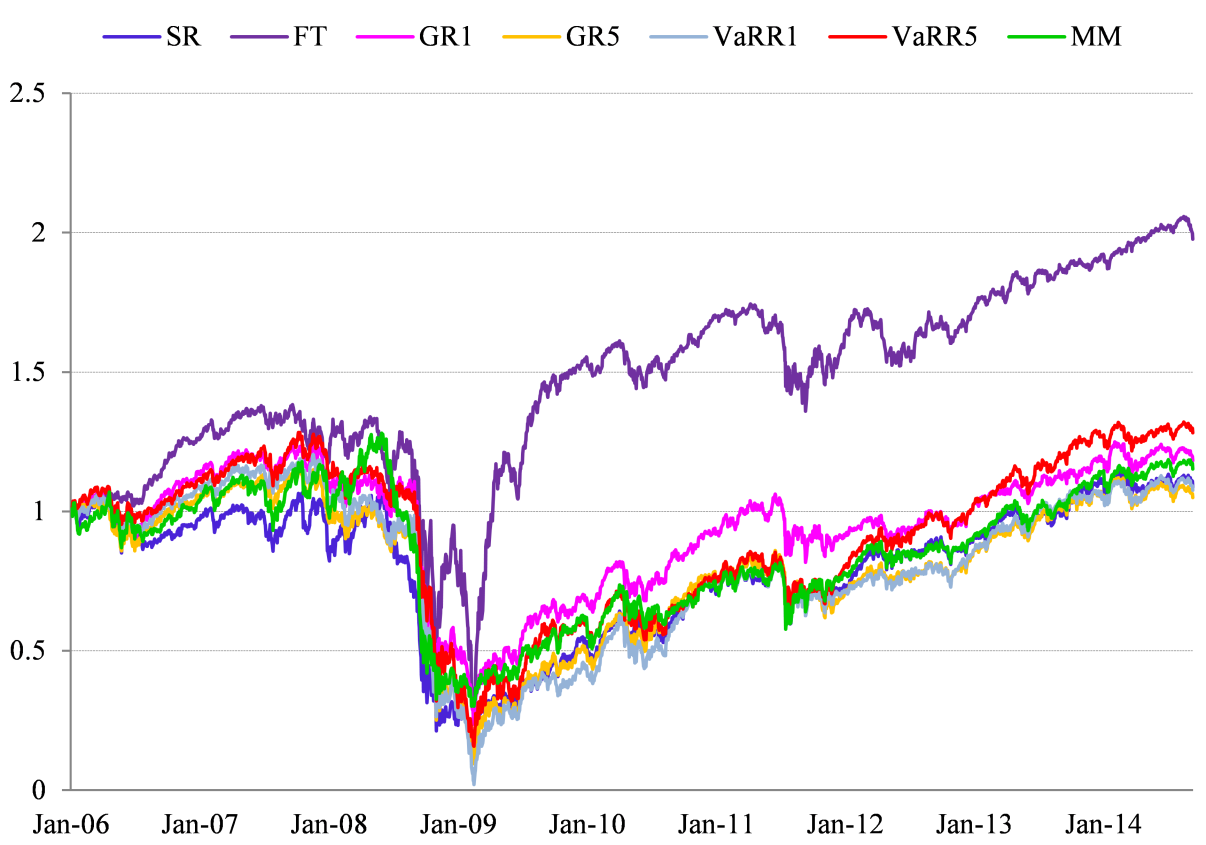
\includegraphics[height=6cm,width=9cm]{texdata/LegacyCumReturns.png}} 
     \label{fig:1} 
  \end{figure}
\end{frame}

\begin{frame}{The Idea: Legacy Research}
  \begin{figure}
    \centering
    \subfloat[Cumulative Wealth of (replicating Strategy) SP500\label{fig:b}]{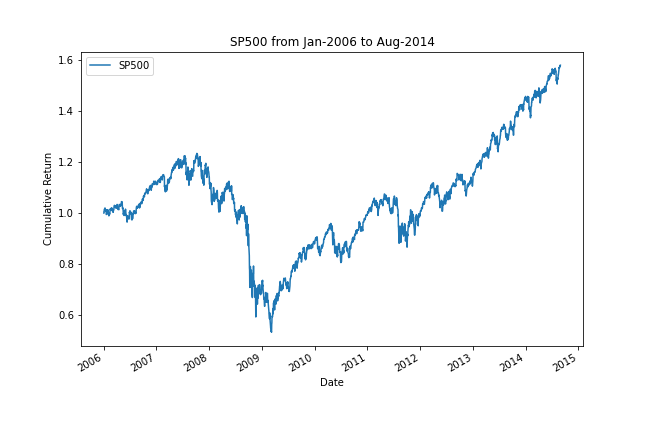
\includegraphics[height=6cm,width=9cm]{texdata/SP500CumReturns.png}}
     \label{fig:LTR1}
  \end{figure}

\end{frame}

\begin{frame}{{\bf LTR} in a Nutshell}
  \begin{figure}
    \centering
    \subfloat[Query (Rebalance Event), Documents (Stocks),
      Rankings\label{fig:LTRa}]{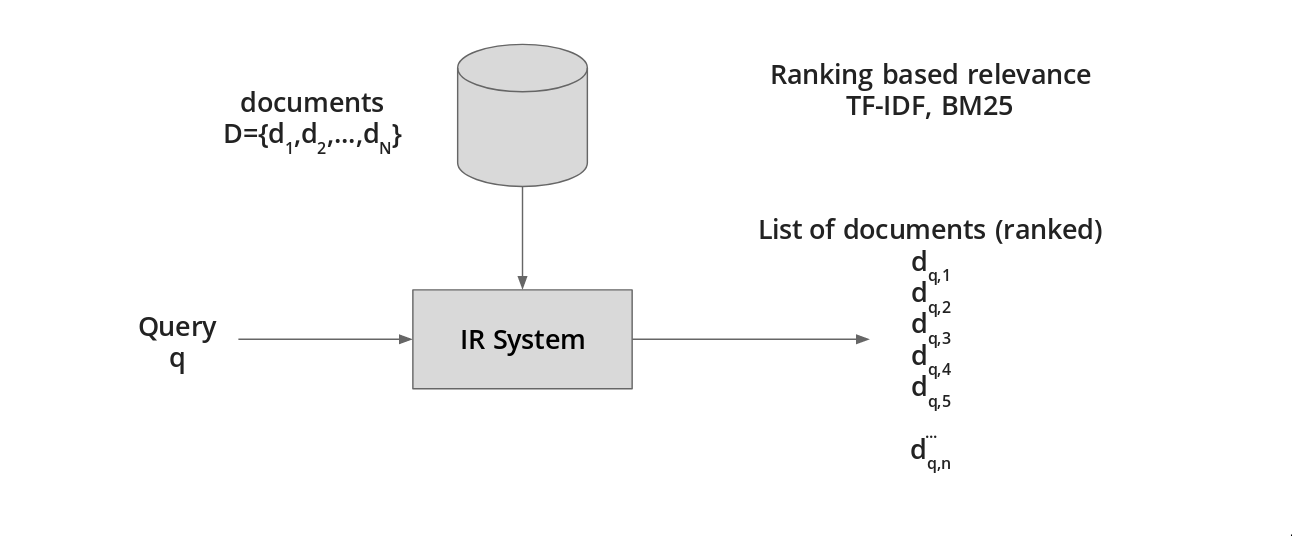
\includegraphics[height=4cm,width=6cm]{texdata/LTR_nutshell.png}}   
        \subfloat[LTR execution flow\label{fig:LTRb}]{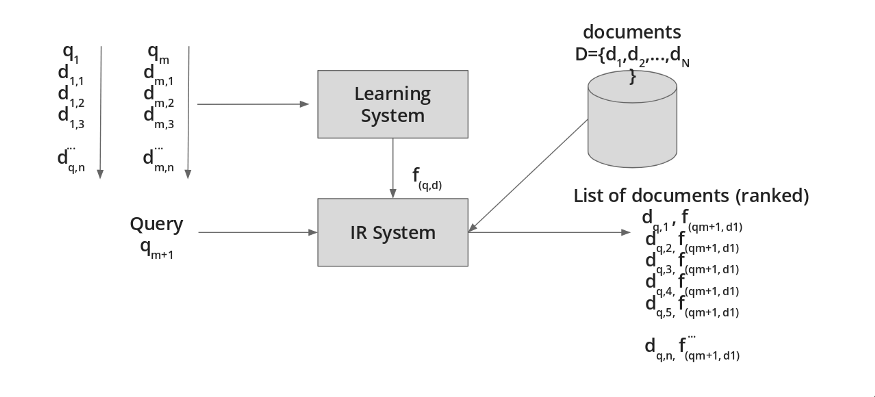
\includegraphics[height=4cm,width=6cm]{texdata/LTR_execution_flow.png}}    
     \label{fig:2}
  \end{figure}
\end{frame}

\section{Dataset}
\begin{frame}{Data}
  \begin{block}{The Dataset}
    \begin{itemize}
    \item Daily {\bf end-of-day quotes}, {\bf market capitalizations}
      and {\bf other} financial information publicly available
      information of the stocks composing S\&P500 (EUROSTOXX600).
      
    \item {\bf Maximum Time-Series Period}: The maximum possible avoiding
      delisting effects. {\sl Estimated:} January 2005-Now

    \item {\bf Source and Methodology:} Yahoo Finance public API
      (Python library {\tt yfinance}, MIT licence) and Web Scrapping
      of {\tt Y! Finance, Wikipedia} ({\tt marketscreener}) websites
      for stock lists.
      \item ICYMI: {\tt nasdaqdatalink, alphavantage} APIs. E.g. {\tt
        quandl (nasdaqdatalink)} free database {\tt WIKI\textbackslash
          PRICES} w/ 1,000 stock historical series. 
    \item {\bf Remark:} {\tt Kaggle} datasets already exist. Avoided
      from the beginning.
    \end{itemize}
    \end{block}

  \begin{block}{Preliminar Exploratory Analysis}
\begin{itemize}
    \item Significant {\bf non-gaussianity} for all stock returns are
      found: this fact motivates the use of Alternative {\bf PMs} as
      predictors.
    \item Individual stocks: Serial correlation for higher moments
      $r^n_t$, uncorrelated raw returns $r_t$.
    \item Strong cross-correlation between some different assets
    \item Some assets behave ``very similar''.
\end{itemize}
\end{block}
  
\end{frame}

\section{The Goal of the Project}
\begin{frame}{What We Search}
  \begin{block}{Targets}
    \begin{itemize}
      \item Show if {\bf PMs} (individual or simple combinations) are
        relevant for Portfolio Construction and Wealth Management.
        \item {\bf Predict Scores} and then {\bf Rankings of Relevant
          Assets} in order to design dynamic Portfolio Rebalancing
          Strategies based on these relevances.
          \item Construct a Frontend showing the Realised
            (track-record) and predicted metrics (financial or
            data-science driven), etc.
            
            In sum, {\bf develop a KID (Key Information Dashboard)}
            summaryzing all the relevant (future and realized)
            financials including portfolio selection. 
      \end{itemize}
    \end{block}
  \begin{block}{State-Of-The-Art}
    \underline{Finance:}
    \begin{itemize}
    \item Very scarce works.
    \item Features based on a simple combination of Technical
      Indicators (rolling simple stats of returns $f(\mathrm{prices})$).
    \item New Sentiment indicators (as features/predictors).
    \end{itemize}
    \underline{Data Science:}
    \begin{itemize}
      \item Out of the Original Scope: A Novel or Less-Known application.
      \end{itemize}
    \end{block}
\end{frame}

\subsection{Technologies and Targets}
\begin{frame}{Technologies}
  \begin{block}{Main technical bullets}
    \begin{description}
    \item[Data Acquisition and Wrangling]: {\tt yfinance
      (nasdaqdatalink, alphavantage), pandas} 
    \item[Exploratory (Time-Series) Data Analysis]: {\tt statmodels,
      arima, pd, matplotlib, sns}
    \item[Supervised LTR (Modeling)]:
      \begin{itemize}
      \item {\sl Pairwise}:  {\sc RankNet} {\tt (keras-tf)} Deep Learning,
        {\sc LambdaMART} {\tt (XGBoost)} 
      \item {\sl Listwise}: {\sc ListNet, ListMLE} {\tt (tf)}, Deep Learning
      \item {\sl All In}: {\tt pytorchltr (torch)}, Deep Learning
      \end{itemize}
      
    \item[Frontend]: Financial Dashboard with Key Information (KID) {\tt (streamlit)}
    \end{description}
  \end{block}

  \begin{block}{Expected Results}
    \begin{itemize}
    \item Significative gain over Heuristical-based Portfolio Rebalancing
    \item A ML-based recommender supported by sofisticated PMs
      (provided by Risk Management literature) as features (not technical indicators). 
    \item A nice/clear KID to help invest/hedge decisions: Equity Desk
        (superhedging, CIB recommendations), Private Banking (retail recommendations) 
    \end{itemize}
  \end{block}
\end{frame}


\subsection{Disaster Recovery Plan}
\begin{frame}{Recovery Plan}
  \begin{block}{Disaster Recovery Plan}
    \begin{description}
    \item[Data:]
      \begin{itemize}
      \item Insufficient data or too many delisting/additions
        (survivorship bias): SP500 $\to$ STOXX600 $\to$ {\tt
        WIKI\textbackslash PRICES} (and change bench) or {\tt
        alphavantage} API.
      \item Last Resource: Use {\tt Kaggle} dataset (updated
        daily) with a complete analysis of the survivors on the
        time sample given.
      \end{itemize}
    \item[Modeling:] Empirical Results not conclusive (or {\bf LTR} not suitable
        for the problem).  
      \begin{itemize}
      \item Try {\bf R-t-R} (regress then rank).
      \item {\bf Techs:} {\sc LSTM, CNN} {\tt (torch, tf)} (RNN, Deep
        Learning)
        \item Last Resource: Regress or Classify (Forecast) SP500
          (index) or representative stocks. 
      \end{itemize}
    \end{description}
  \end{block}
\end{frame}


\subsection{Time Schedule}
\begin{frame}{Schedule}
  \centering
  \ovalbox{Mandatory update and/or reschedule each end-of-week}
  \begin{block}{Time Schedule}
    \begin{description}
    \item[Data:] Jul-25/Aug-12 (3w)
      \begin{itemize}
      \item Managing Delisting/Addtions,
      \item EDA raw-returns,
      \item Features ({\bf PMs}) construction, analysis
        (dimensionality reduction)
      \end{itemize}
    \item[Modeling, Part I (MVP):] Aug-16/Sep-09 (3w, 1 week-out)
      \begin{itemize}
      \item Understand LTR basics (algorithm, metrics).
      \item Accurate mapping of the [Queries,Relevant Documents] to
        the Intertemporal Portfolio problem: [Rebalance Events,Relevant Assets]
      \item Implement {\sc RankNet}
      \item Empirical Analysis. Conclusions. KID Prototype. Memo guidelines.
      \end{itemize}
      \item[Modeling, Part II (Generalization):] Sep-12/Oct-07 (4w)
        \begin{itemize}
        \item Rest of the LTR Implementations (pairwise \& listwise).
        \item Empirical comparison with benchmark (random/naive
          baselines)
        \item KID generalisation. Memo final skeleton
        \end{itemize}
      \item[Final Stage, KID (Frontend)] Oct-10/Nov-11 (5w)
        \begin{itemize}
        \item Design-Test final KID.
        \item Memo/Presentation
        \end{itemize}

    \end{description}
  \end{block}
\end{frame}

\section{Referencias}
\begin{frame}{Referencias}
  \begin{thebibliography}{9}
      \bibitem{NAJEF2019} Le\'on et al. (2019), Screening Rules and Portfolio
        Performance. \emph{North American Journal of Economics and
        Finance} 
  \bibitem{JBF2020} Le\'on et al. (2020), Modeling asset returns under
  time-varying semi-nonparametric distributions, \emph{Journal of
  Banking and Finance}. 
  \bibitem{Giles2008} Poh et al., (2022). Enhancing
    Cross-Sectional Currency Strategies by Context-Aware Learning to
    Rank with Self-Attention. \emph{The Journal of Financial Data
    Science}
\bibitem{Song2017} Song, et al., (2017). Stock Portfolio Selection
  Using Learning-to-Rank Algorithms with News Sentiments, \emph{Neurocomputing}
  \end{thebibliography}
\end{frame}

\begin{frame}{Thanks!}
  \begin{figure}
    \centering
    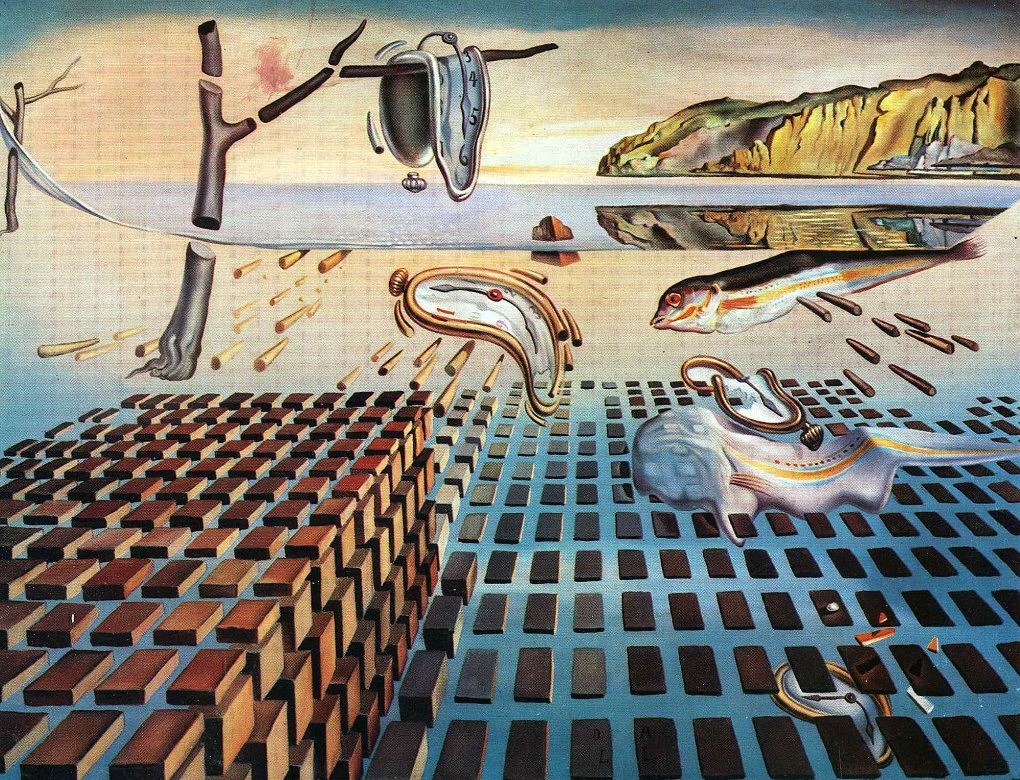
\includegraphics[height=6.5cm,width=6.5cm]{texdata/PersistenceMemory.jpg}\caption{La Persist\`encia de la Mem\`oria.}
  \end{figure}
  
\end{frame}

\end{document}

%% \begin{block}{Fundamentales}
%%   \[
%% \begin{cases}
%% \alpha(t) = e^{a t}\sigma(t) \\
%% \zeta(t) = \int_0^t\alpha_s^2ds =
%% \int_0^te^{2a s}\sigma_s^2ds\\
%% H(t) = \int_0^te^{-a s}ds.\\
%% N(t) =
%% \frac{1}{P(0,t)}\exp\left\{H(t)X_t+\frac{1}{2}H^2(t)\zeta(t)\right\}\\
%% P(t,T) = \frac{P(0,T)}{P(0,t)}\exp\left\{- [H(T) - H(t)]X_t -
%% \frac{1}{2}[H^2(T) - H^2(t)]\zeta_t\right\}
%% \end{cases}
%% \]
%% \end{block}
%% Hay m\'ultiples alternativas para calibrar ($\zeta(t)$, $H(t)$):
%% \begin{itemize}
%% \item Se
%% fija $H(t)$ mediante su relaci\'on con un HW con $a$ constante
%% (calibrado a $N$ caplets). Se deshecha $\sigma_{HW}$ (preset {\sc Analytics}).
%% \item Con $N$ caplets se calibra la funci\'on $\zeta(t_i)$ con $t_i=
%%   \tau, 2\tau,\dots, T_{max}$, el mallado temporal que nos interese.
%% \end{itemize}
%% Con $\zeta(t)$ y $H(t)$ definidos ya se puede simular $N(t)$ y
%% $P(t,T)$.

%\section{Calibraci\'on}
%\subsection{Caplet Stripping}
%% \begin{frame}{Calibraci\'on con Caplets}
%% Tipo Libor para periodo $[T_s, T_e]$, con {\sl fixing} en  $t_f \le
%% T_s$.
%% caplet con strike $K$ y tenor para el mismo per\'\i odo $[T_s, T_e]$, $\tau$.
%% F\'ormula cerrada para caplet basado en LGM unifactorial
%% \[
%% \boxed{V_0^{LGM} = P(0,T_e)\tau \mbox{Bl}\left(K+\frac{1}{\tau}, F+\frac{1}{\tau}, \left[H(T_e)-H(T_s)\right] \sqrt{\zeta_{t_f}}, 1\right)}
%% \]
%% donde $H(t) = \frac{1-e^{-a t}}{a}$ (precalibrado HW), $\zeta(t) = \int_0^t \alpha^2(s) ds$ y
%% $\mbox{Bl}(K,F,v,\omega)$ viene dado
%% \[
%% \mbox{Bl}(K,F,v,\omega)=F\omega\Phi(\omega d_1) - K\omega\Phi(\omega
%% d_2), \; d_1 =
%% \frac{\ln(F/K)+v^2/2}{v}, \; d_2 = \frac{\ln(F/K)-v^2/2}{v}
%% \]
%% Calibraci\'on con caplets para obtener $\zeta_{t_f}$ requiere resolver
%% recurrentemente $\forall~t_f$: 
%% \[ 
%% \boxed{
%% \mathcal{N}\mbox{Bl}(K, F, \sigma_N \sqrt{t_f}, 1) = \mbox{Bl}\left(K+\frac{1}{\tau}, F+\frac{1}{\tau}, \left[H(T_e)-H(T_s)\right] \sqrt{\zeta_{t_f}}, 1\right),
%% }
%% \]
%% donde: % $\mathcal{N}{Bl}(K,F,v,\omega)$ viene dado
%% \[
%%   \mathcal{N}\mbox{Bl}(K,F,\nu,\omega)=\nu\phi(d) + \omega (F-K)
%%   \Phi(\omega d)\quad d =\frac{F-K}{\nu}\,.
%% \]
%% \ovalbox{El mercado cotiza par (flat) volatilities $\bar{\sigma}_N$ de
%%   caps para varios strikes: {\sl stripping.} $\bar{\sigma}_N \to \sigma_N$.}
%% \end{frame}

%% \begin{frame}{Calibraci\'on con Caplets (stripping)}
%% Stripping:
%%   $$
%% \boxed{  C_n(\bar{\sigma}_n,\boldsymbol{\theta})
%%   =\sum_{i}^{M(n)}c_i(\sigma_i,\boldsymbol{\theta})\qquad
%% n=1,\dots,N\;\text{n\'umero caps} }
%%   $$
%% e.g. Cap 2y con $\tau = 0.25$, $M(n)=M/\tau-1=7$.
%% \begin{figure}
%%     \centering
%%     \subfloat[Market TSV of Caps\label{fig:a}]{\includegraphics[height=4cm,width=4cm]{texdata/TSVCaps.jpg}}\qquad 
%%     \subfloat[Stripped TSV of Caplets\label{fig:b}]{\includegraphics[height=4cm,width=4cm]{texdata/TSVCaplets.jpg}}
%%     \caption{Caplet Stripping con MDA, $K=0$.}
%%     \label{fig:1}
%%   \end{figure}
%% \end{frame}


%% \begin{frame}{Calibraci\'on con Caplets (resultados)}
%%   \centering
%% %\framebox{\large  Stripping 30/11/2018:}
%%   \begin{description}
%%   \item[HW:] $\left(a_{HW}=0.4377\%,\sigma_{HW}=0.5538\% \right)$
%%   \item[LGM:] $\left( H(t)= f(a_{HW}), \zeta(\cdot) \to
%%       \zeta_1,\zeta_2,\dots,\zeta_{nlets} \right)$
%%   \end{description}
  
%% \begin{figure}
%%     \centering
%%     \subfloat[HW Caplet Calibration Absolute Error
%%     (bp)\label{fig:a}]{\includegraphics[height=4cm,width=4cm]{texdata/ErrorCapletsHW.jpg}}\qquad    
%%     \subfloat[$\zeta_{HW}$ versus
%%     $\zeta_{LGM}$\label{fig:b}]{\includegraphics[height=4cm,width=4cm]{texdata/ZetaHWvsZetaLGM.jpg}} 
%%     \caption{Calibraci\'on Caplets con $K=0$. $\zeta_{HW} = \sigma^2
%%       \frac{1-exp(-2 a t)}{2 a}\approx \sigma^2 t$.} 
%%     \label{fig:1}
%%   \end{figure}
%% \end{frame}

%\subsection{Resultados: Quality Checks en PVs de Caplets}
%% \begin{frame}{Simulaci\'on (resultados)}
%% \begin{figure}
%%     \centering
%%     \includegraphics[height=6cm,width=7.5cm]{ValErrorQMC.jpg}% \qquad
%%     % \subfloat[Secuencia bidimensional pseudoaleatoria\label{fig:b}]{\includegraphics[height=5cm,width=5cm]{pseudornd_2.jpg}}
%%     \caption{QMC con $N_{sim}=10\,000$ y Variables Antit\'eticas. Error en (bp).}
%%     \label{fig:1}
%%   \end{figure}
%% \end{frame}


%% \begin{frame}{Esquema Engine para DRV}
%% \centering
%%     \begin{tikzpicture}
%%           [node distance=.5cm,
%%   start chain=going below,]
%%      \node[punktchain, join] (intro) {MDA: {\tt Panorama}, {\tt CorbesEuribor}};
%%      \node[punktchain, join] (Calib)      {(Re)Calibraci\'on $H,\zeta$};
%%      \node[punktchain, join] (investeringer) {Simulaci\'on};
%%      \node[punktchain, join] (Bump) {Bumping $\sigma$};
%%      \node[punktchain, join, ] (emperi) {Outputs DRV:\\($D$, $D_f$) y $(D^\sigma_\pm, D^\sigma_{f,\pm})$};
%%        \draw [->] (Bump.east) -| (Calib.east);
%%   \end{tikzpicture}
%% \end{frame}
